\section*{How to Use This Book: Section Roadmaps}
\addcontentsline{toc}{section}{How to Use This Book: Section Roadmaps}

This book presents the Elder Theory framework through a structured progression from foundational concepts to practical applications. To help navigate this complex material, we provide visual roadmaps showing where each major section fits within the overall framework.

\subsection*{Overall Structure}

The book is organized into seven theoretical sections followed by an experimental section:

\begin{figure}[h]
\centering
\begin{tikzpicture}[roadmap/.style={rectangle, draw, fill=blue!10, text width=3.5cm, minimum height=1cm, align=center}, arrow/.style={->, thick, >=stealth}, node distance=1.5cm]
    % Sections
    \node[roadmap, fill=yellow!20] (s1) {I. Foundation Layer};
    \node[roadmap, fill=yellow!30, below=of s1] (s2) {II. Core Mathematical Framework};
    \node[roadmap, fill=yellow!40, below=of s2] (s3) {III. Hierarchical Learning Structure};
    \node[roadmap, fill=yellow!50, below=of s3] (s4) {IV. Loss Functions by Component};
    \node[roadmap, fill=yellow!60, below=of s4] (s5) {V. Complete Algorithm};
    \node[roadmap, fill=yellow!70, below=of s5] (s6) {VI. Unified System Theory};
    \node[roadmap, fill=yellow!80, below=of s6] (s7) {VII. Domain Applications};
    \node[roadmap, fill=green!30, below=of s7] (s8) {Experiments};
    
    % Arrows
    \draw[arrow] (s1) -- (s2);
    \draw[arrow] (s2) -- (s3);
    \draw[arrow] (s3) -- (s4);
    \draw[arrow] (s4) -- (s5);
    \draw[arrow] (s5) -- (s6);
    \draw[arrow] (s6) -- (s7);
    \draw[arrow] (s7) -- (s8);
    
    % Annotations
    \node[right=0.5cm of s1, text width=6cm] {Abstract mathematical spaces};
    \node[right=0.5cm of s2, text width=6cm] {Heliomorphic functions and manifolds};
    \node[right=0.5cm of s3, text width=6cm] {Elder-Mentor-Erudite organization};
    \node[right=0.5cm of s4, text width=6cm] {Learning mechanisms at each level};
    \node[right=0.5cm of s5, text width=6cm] {Synthesis into operational algorithm};
    \node[right=0.5cm of s6, text width=6cm] {Integration into complete system};
    \node[right=0.5cm of s7, text width=6cm] {Applications across domains};
    \node[right=0.5cm of s8, text width=6cm] {Empirical validation};
\end{tikzpicture}
\caption{Overall progression of sections in the Elder Theory book}
\label{fig:overall_roadmap}
\end{figure}

\subsection*{Section I: Foundation Layer}

\begin{figure}[h]
\centering
\begin{tikzpicture}[
    highlight/.style={rectangle, draw, fill=yellow!20, text width=3.5cm, minimum height=1cm, align=center},
    normal/.style={rectangle, draw, fill=blue!10, text width=3.5cm, minimum height=1cm, align=center, opacity=0.5},
    arrow/.style={->, thick, >=stealth}, 
    node distance=1.5cm
]
    % Sections
    \node[highlight] (s1) {I. Foundation Layer};
    \node[normal, below=of s1] (s2) {II. Core Mathematical Framework};
    \node[normal, below=of s2] (s3) {III. Hierarchical Learning Structure};
    \node[normal, below=of s3] (s4) {IV. Loss Functions by Component};
    \node[normal, below=of s4] (s5) {V. Complete Algorithm};
    \node[normal, below=of s5] (s6) {VI. Unified System Theory};
    \node[normal, below=of s6] (s7) {VII. Domain Applications};
    \node[normal, below=of s7] (s8) {Experiments};
    
    % Arrows
    \draw[arrow] (s1) -- (s2);
    \draw[arrow, opacity=0.5] (s2) -- (s3);
    \draw[arrow, opacity=0.5] (s3) -- (s4);
    \draw[arrow, opacity=0.5] (s4) -- (s5);
    \draw[arrow, opacity=0.5] (s5) -- (s6);
    \draw[arrow, opacity=0.5] (s6) -- (s7);
    \draw[arrow, opacity=0.5] (s7) -- (s8);
    
    % Chapter details
    \node[rectangle, draw, fill=green!20, text width=4cm, align=center, right=1.5cm of s1] (c1) {Concrete Example};
    \node[rectangle, draw, fill=yellow!20, text width=4cm, align=center, right=1.5cm of c1] (c2) {Introduction to Elder Spaces};
    \node[rectangle, draw, fill=yellow!20, text width=4cm, align=center, below=0.5cm of c2] (c3) {Introduction to Elder Topology};
    
    % Connect chapters to section
    \draw[arrow] (s1) -- (c1);
    \draw[arrow] (c1) -- (c2);
    \draw[arrow] (c2) -- (c3);
    
    % Chapter descriptions
    \node[below right=-0.1cm and 0.2cm of c1.south east, text width=3cm, font=\small, align=left] {Practical example that grounds abstract concepts};
    \node[below right=-0.1cm and 0.2cm of c2.south east, text width=3cm, font=\small, align=left] {Abstract spaces for knowledge representation};
    \node[below right=-0.1cm and 0.2cm of c3.south east, text width=3cm, font=\small, align=left] {Mappings between abstract and concrete};
\end{tikzpicture}
\caption{Section I: Foundation Layer}
\label{fig:section1_roadmap}
\end{figure}

\subsection*{Section II: Core Mathematical Framework}

\begin{figure}[h]
\centering
\begin{tikzpicture}[
    highlight/.style={rectangle, draw, fill=yellow!30, text width=3.5cm, minimum height=1cm, align=center},
    normal/.style={rectangle, draw, fill=blue!10, text width=3.5cm, minimum height=1cm, align=center, opacity=0.5},
    arrow/.style={->, thick, >=stealth}, 
    node distance=1.5cm
]
    % Sections
    \node[normal] (s1) {I. Foundation Layer};
    \node[highlight, below=of s1] (s2) {II. Core Mathematical Framework};
    \node[normal, below=of s2] (s3) {III. Hierarchical Learning Structure};
    \node[normal, below=of s3] (s4) {IV. Loss Functions by Component};
    \node[normal, below=of s4] (s5) {V. Complete Algorithm};
    \node[normal, below=of s5] (s6) {VI. Unified System Theory};
    \node[normal, below=of s6] (s7) {VII. Domain Applications};
    \node[normal, below=of s7] (s8) {Experiments};
    
    % Arrows
    \draw[arrow, opacity=0.5] (s1) -- (s2);
    \draw[arrow] (s2) -- (s3);
    \draw[arrow, opacity=0.5] (s3) -- (s4);
    \draw[arrow, opacity=0.5] (s4) -- (s5);
    \draw[arrow, opacity=0.5] (s5) -- (s6);
    \draw[arrow, opacity=0.5] (s6) -- (s7);
    \draw[arrow, opacity=0.5] (s7) -- (s8);
    
    % Chapter details
    \node[rectangle, draw, fill=yellow!30, text width=4cm, align=center, right=1.5cm of s2] (c1) {Heliomorphic Functions};
    \node[rectangle, draw, fill=yellow!30, text width=4cm, align=center, below=0.5cm of c1] (c2) {Elder Manifold};
    \node[rectangle, draw, fill=yellow!30, text width=4cm, align=center, below=0.5cm of c2] (c3) {Heliomorphic Geometry};
    \node[rectangle, draw, fill=yellow!30, text width=4cm, align=center, below=0.5cm of c3] (c4) {Heliomorphism};
    
    % Connect chapters to section
    \draw[arrow] (s2) -- (c1);
    \draw[arrow] (c1) -- (c2);
    \draw[arrow] (c2) -- (c3);
    \draw[arrow] (c3) -- (c4);
    
    % Chapter descriptions
    \node[below right=-0.1cm and 0.2cm of c1.south east, text width=4cm, font=\small, align=left] {Distinct mathematical framework};
    \node[below right=-0.1cm and 0.2cm of c2.south east, text width=4cm, font=\small, align=left] {Geometric structure for knowledge};
    \node[below right=-0.1cm and 0.2cm of c3.south east, text width=4cm, font=\small, align=left] {Mathematical basis with radial dynamics};
    \node[below right=-0.1cm and 0.2cm of c4.south east, text width=4cm, font=\small, align=left] {Application to learning systems};
\end{tikzpicture}
\caption{Section II: Core Mathematical Framework}
\label{fig:section2_roadmap}
\end{figure}

\subsection*{Section III: Hierarchical Learning Structure}

\begin{figure}[h]
\centering
\begin{tikzpicture}[
    highlight/.style={rectangle, draw, fill=yellow!40, text width=3.5cm, minimum height=1cm, align=center},
    normal/.style={rectangle, draw, fill=blue!10, text width=3.5cm, minimum height=1cm, align=center, opacity=0.5},
    arrow/.style={->, thick, >=stealth}, 
    node distance=1.5cm
]
    % Sections
    \node[normal] (s1) {I. Foundation Layer};
    \node[normal, below=of s1] (s2) {II. Core Mathematical Framework};
    \node[highlight, below=of s2] (s3) {III. Hierarchical Learning Structure};
    \node[normal, below=of s3] (s4) {IV. Loss Functions by Component};
    \node[normal, below=of s4] (s5) {V. Complete Algorithm};
    \node[normal, below=of s5] (s6) {VI. Unified System Theory};
    \node[normal, below=of s6] (s7) {VII. Domain Applications};
    \node[normal, below=of s7] (s8) {Experiments};
    
    % Arrows
    \draw[arrow, opacity=0.5] (s1) -- (s2);
    \draw[arrow, opacity=0.5] (s2) -- (s3);
    \draw[arrow] (s3) -- (s4);
    \draw[arrow, opacity=0.5] (s4) -- (s5);
    \draw[arrow, opacity=0.5] (s5) -- (s6);
    \draw[arrow, opacity=0.5] (s6) -- (s7);
    \draw[arrow, opacity=0.5] (s7) -- (s8);
    
    % Chapter details
    \node[rectangle, draw, fill=yellow!40, text width=4cm, align=center, right=1.5cm of s3] (c1) {Hierarchical Knowledge Architecture};
    
    % Connect chapters to section
    \draw[arrow] (s3) -- (c1);
    
    % Chapter descriptions
    \node[below right=-0.1cm and 0.2cm of c1.south east, text width=6cm, font=\small, align=left] {Complete system architecture with Elder-Mentor-Erudite organization and interactions};
\end{tikzpicture}
\caption{Section III: Hierarchical Learning Structure}
\label{fig:section3_roadmap}
\end{figure}

These roadmaps continue for each section, providing a visual guide to the book's structure and helping readers understand how individual chapters contribute to the overall framework.

\begin{figure}[h]
\centering
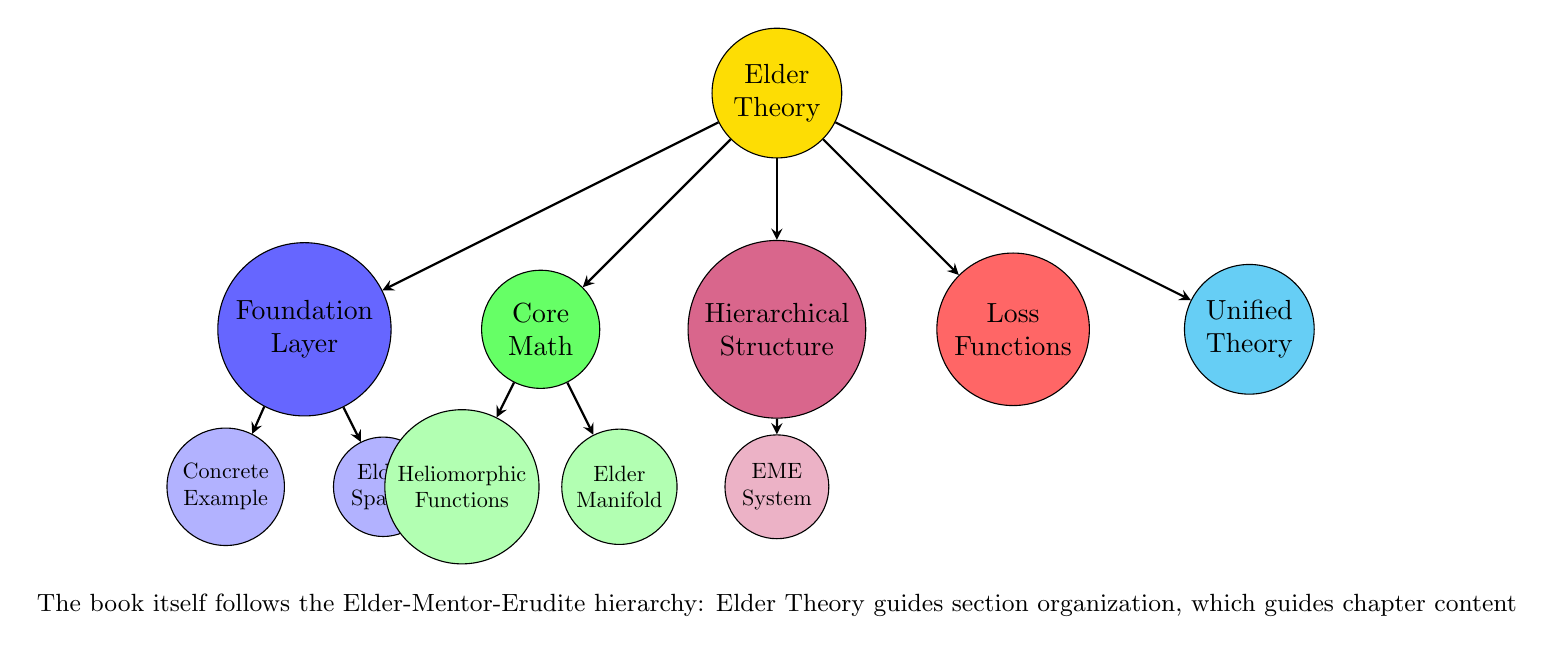
\begin{tikzpicture}[
    entity/.style={circle, draw, minimum size=1.5cm, align=center},
    arrow/.style={->, thick, >=stealth}, 
    label/.style={font=\small, align=center}
]
    % Elder
    \node[entity, fill=yellow!80!orange] (elder) at (0,0) {Elder\\Theory};
    
    % Sections as Mentors
    \node[entity, fill=blue!60] (s1) at (-6,-3) {Foundation\\Layer};
    \node[entity, fill=green!60] (s2) at (-3,-3) {Core\\Math};
    \node[entity, fill=purple!60] (s3) at (0,-3) {Hierarchical\\Structure};
    \node[entity, fill=red!60] (s4) at (3,-3) {Loss\\Functions};
    \node[entity, fill=cyan!60] (s5) at (6,-3) {Unified\\Theory};
    
    % Chapters as Erudites (just a few shown for clarity)
    \node[entity, fill=blue!30, scale=0.8] (c1) at (-7,-5) {Concrete\\Example};
    \node[entity, fill=blue!30, scale=0.8] (c2) at (-5,-5) {Elder\\Spaces};
    
    \node[entity, fill=green!30, scale=0.8] (c3) at (-4,-5) {Heliomorphic\\Functions};
    \node[entity, fill=green!30, scale=0.8] (c4) at (-2,-5) {Elder\\Manifold};
    
    \node[entity, fill=purple!30, scale=0.8] (c5) at (0,-5) {EME\\System};
    
    % Connections
    \draw[arrow] (elder) -- (s1);
    \draw[arrow] (elder) -- (s2);
    \draw[arrow] (elder) -- (s3);
    \draw[arrow] (elder) -- (s4);
    \draw[arrow] (elder) -- (s5);
    
    \draw[arrow] (s1) -- (c1);
    \draw[arrow] (s1) -- (c2);
    \draw[arrow] (s2) -- (c3);
    \draw[arrow] (s2) -- (c4);
    \draw[arrow] (s3) -- (c5);
    
    % Labels
    \node[label] at (0,-6.5) {The book itself follows the Elder-Mentor-Erudite hierarchy: Elder Theory guides section organization, which guides chapter content};
\end{tikzpicture}
\caption{The book's structure as an Elder Heliosystem}
\label{fig:book_as_heliosystem}
\end{figure}

Use these roadmaps to navigate the material and understand how each component contributes to the complete Elder Theory framework.